\documentclass[whitelogo]{TUD-report2020}

\usepackage[style=apa]{biblatex}
\addbibresource{report.bib}

\usepackage{changes}
\begin{document}

%% Use Roman numerals for the page numbers of the title pages and table of
%% contents.
\frontmatter

%% Uncomment following 19 lines for a cover with a picture on the lower half only
%\title[tudelft-white]{Title}
%\subtitle[tudelft-cyan]{Optional subtitle}
%\author[tudelft-white]{J.\ Random Author}
%\affiliation{Technische Universiteit Delft}
%\coverimage{cover.jpg}
%\titleoffsetx{10cm}
%\titleoffsety{10cm}
%\afiloffsetx{1cm}
%\afiloffsety{18cm}
%\covertext[tudelft-white]{
%    \textbf{Cover Text} \\
%    possibly \\
%    spanning 
%    multiple 
%    lines
%    \vfill
%    ISBN 000-00-0000-000-0
%}
%\makecover

%% Uncomment following 16 lines for a cover with a picture on the lower half only
\title[tudelft-white]{MSc Graduation Guide}
\subtitle[tudelft-black]{at KAS Lab}
\author[tudelft-white]{Knowledge-based Autonomous Systems Laboratory}
\affiliation{Technische Universiteit Delft}
% \coverimage{tank.jpg}
\coverimage{figures/DALL_E_20221222_robotreadingaboutknowledgerepresentationandsymbolicreasoning.jpg}
\covertext[tudelft-white]{
    \textbf{Authors:} \\
    Carlos Hernandez Corbato
    \vfill
    Date 2022-12-22
}
\setpagecolor{tudelft-cyan}
\makecover[split]


%% Include an optional title page.
\begin{titlepage}


\begin{center}

%% Insert the TU Delft logo at the bottom of the page.

%% Print the title in cyan.
{\makeatletter
\largetitlestyle\fontsize{64}{94}\selectfont\@title
%\largetitlestyle\color{tudelft-cyan}\Huge\@title
\makeatother}

%% Print the optional subtitle in black.
{\makeatletter
\ifx\@subtitle\undefined\else
    \bigskip
   {\tudsffamily\fontsize{22}{32}\selectfont\@subtitle}    
    %\titlefont\titleshape\LARGE\@subtitle
\fi
\makeatother}

\bigskip
\bigskip

by
%door

\bigskip
\bigskip

%% Print the name of the author.
{\makeatletter
%\largetitlefont\Large\bfseries\@author
\largetitlestyle\fontsize{26}{26}\selectfont\@author
\makeatother}

\bigskip
\bigskip

% to obtain the degree of Master of Science
% %ter verkrijging van de graad van Master of Science

% at the Delft University of Technology,
% %aan de Technische Universiteit Delft,

% to be defended publicly on Tuesday January 1, 2013 at 10:00 AM.
%in het openbaar de verdedigen op dinsdag 1 januari om 10:00 uur.

\vfill

% \begin{tabular}{lll}
%     Student number: & 1234567 \\
%     Project duration: & \multicolumn{2}{l}{March 1, 2012 -- January 1, 2013} \\
%     Thesis committee: & Prof.\ dr.\ ir.\ J.\ Doe, & TU Delft, supervisor \\
%         & Dr.\ E.\ L.\ Brown, & TU Delft \\
%         & Ir.\ A.\ Aaronson, & Acme Corporation
% \end{tabular}
%% Only include the following lines if confidentiality is applicable.

\bigskip
\bigskip
\emph{license text}
%\emph{Op dit verslag is geheimhouding van toepassing tot en met 31 december 2013.}

\bigskip
\bigskip
An electronic version of this document is available at \url{http://}.
%\\[1cm]

%\centering{
\includegraphics{cover/logo_black}}


\end{center}

\begin{tikzpicture}[remember picture, overlay]
    \node at (current page.south)[anchor=south,inner sep=0pt]{
        
\includegraphics{cover/logo_black}
    };
\end{tikzpicture}

\end{titlepage}



% \chapter*{Preface}
\setheader{Preface}

Preface\ldots

\begin{flushright}
{\makeatletter\itshape
    \@author \\
    Delft, January 2013
\makeatother}
\end{flushright}



\tableofcontents

%% Use Arabic numerals for the page numbers of the chapters.
\mainmatter

\chapter{Introduction}

\section{Who is this guide for?}

This document has been written for master students intending to graduate at the KAS Laboratory, section Robot Dynamics of the department Cognitive Robotics (Faculty 3mE, TU Delft). Typically, these include MSc students from the MSc Robotics \url{https://www.tudelft.nl/onderwijs/opleidingen/masters/robotics/msc-robotics/programme} or BioMechanical Engineering (specialisations BioRobotics). Exceptionally, we supervise students from other backgrounds as well. 
Nonetheless, the guide contains a lot of general tips and tricks that can be applied in other domains.

Disclaimer: this guide is heavily based on the "Master Thesis Guide
Written by Delft Haptics Lab members" (version June 9 2020). We are very grateful to them for sharing such a beautiful guide, and hope there are ok with us reusing parts of it for the KAS Lab guide.

\section{Why this guide?}

A graduation project is a \textit{process}, and as a student typically you have not done it before.
This process covers most of your second year of your MSc, from finding a thesis supervisor and a topic, to eventuelly presenting and defending your project.

This guide is intended to help you in that process. 

% FROM HRI Manual
% Note that an MSc thesis project is not a straightforward affair to which a step-by-step ‘manual’ can be applied. As such, this guide is no more than a guide, it provides a structured approach, examples, and helpful tips \& tricks, but that does not mean this is the only way to go about your thesis project. Please also make use of other guides, tips, tricks, conversations with students & staff, and of course your own creativity and common sense.

\section{Overview of the graduation process and this guide}

\begin{list}
    % \item Chapter \ref{}
    % \item Chapter \ref{}
    % \item Chapter \ref{}
    % \item Chapter \ref{}
\end{list}

\chapter{Literature Review}\label{c:literature}

\section{What is a Literature Review}
Literature Research is also referred to as Literature Study or Literature Review.
It is individual work on a topic agreed upon between the thesis supervisor and the student.
It involves creating a research question that can be answered using the existing literature, finding and analyzing the right literature, and writing a solid report about it.

% FROM HRI MANUAL
This chapter aims to give guidelines and suggestions to help you in writing your literature report. Typically the report writing takes three months and can roughly be divided into three phases, each requiring approximately one month’s work:
\begin{enumerate}
    \item Orientation \& exploration.
    \item Structured literature search.
    \item Literature documentation.
\end{enumerate}

\begin{figure}[h!]
	\centering
	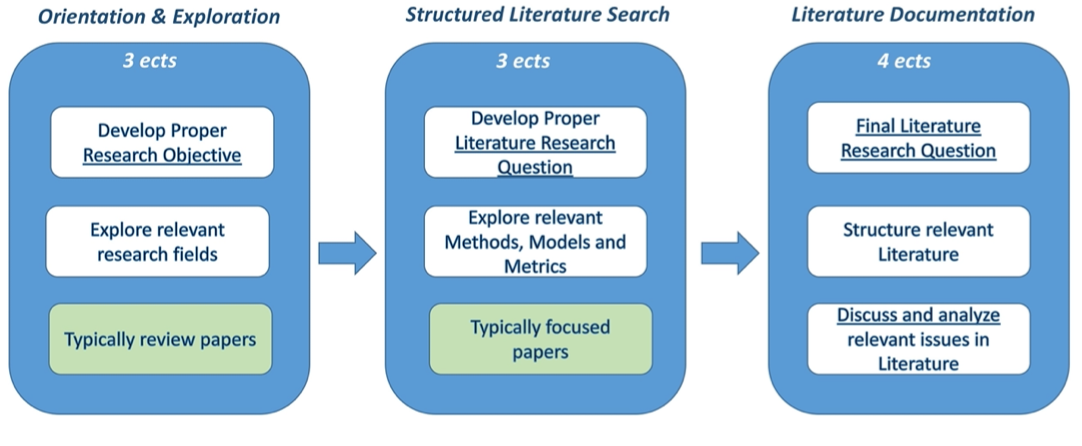
\includegraphics[width=0.8\textwidth]{figures/literatu_study_process.png}
	\caption{Overview of the literature study, reproduced from \cite{Master Thesis Guide, HRI section Cognitive Robotics}.}
	\label{fig:dexnet3_functionality}
\end{figure}

\section{Literature Review in the MSc Robotics program}
The Literature Review is called the Literature Research in the MSc Robotics Program, and it is 10EC
In detail, from the Study Guide \url{https://studiegids.tudelft.nl/}:

\begin{quote}
The aim of the literature study is to learn how to independently search for recent scientific publications (i.e., articles, theses, books). The literature study is carried out individually. The topic of the literature study is linked to the graduation project. The findings from the literature study are used to motivate the research plan of the thesis and are instrumental for achieving a high-quality final thesis.
\end{quote}

Learning Objectives:
After completing their literature research, students will be able to:
\begin{itemize}
    \item study a topic by critically selecting relevant scientific literature,
    \item identify and acquire lacking expertise
    \item identify the most interesting and relevant questions or problems in the field of the MSc thesis
    \item analyse and solve engineering problems in a systematic way
    \item present and report in good English
\end{itemize}

This part of your graduation process includes the following activities which are assessed:
\begin{itemize}
    \item Literature Research (written report; minimum grade: 6.0). The report is graded by the supervisor.
    \item Presentation (colloquium) (pass/fail). The presentation is combined with the introductory phase of the MSc project. The colloquium is graded by an ad-hoc committee of scientific employees of the department.
    \item Colloquium Attendance (pass/fail). All students must attend at least 10 colloquia.
\end{itemize}
	
\section{Literature Review at KAS Lab}


%% Use letters for the chapter numbers of the appendices.
\appendix

%\input{appendix-a}

\printbibliography

\end{document}

